% Options for packages loaded elsewhere
\PassOptionsToPackage{unicode}{hyperref}
\PassOptionsToPackage{hyphens}{url}
%
\documentclass[
  man,floatsintext]{apa6}
\usepackage{amsmath,amssymb}
\usepackage{lmodern}
\usepackage{iftex}
\ifPDFTeX
  \usepackage[T1]{fontenc}
  \usepackage[utf8]{inputenc}
  \usepackage{textcomp} % provide euro and other symbols
\else % if luatex or xetex
  \usepackage{unicode-math}
  \defaultfontfeatures{Scale=MatchLowercase}
  \defaultfontfeatures[\rmfamily]{Ligatures=TeX,Scale=1}
\fi
% Use upquote if available, for straight quotes in verbatim environments
\IfFileExists{upquote.sty}{\usepackage{upquote}}{}
\IfFileExists{microtype.sty}{% use microtype if available
  \usepackage[]{microtype}
  \UseMicrotypeSet[protrusion]{basicmath} % disable protrusion for tt fonts
}{}
\makeatletter
\@ifundefined{KOMAClassName}{% if non-KOMA class
  \IfFileExists{parskip.sty}{%
    \usepackage{parskip}
  }{% else
    \setlength{\parindent}{0pt}
    \setlength{\parskip}{6pt plus 2pt minus 1pt}}
}{% if KOMA class
  \KOMAoptions{parskip=half}}
\makeatother
\usepackage{xcolor}
\IfFileExists{xurl.sty}{\usepackage{xurl}}{} % add URL line breaks if available
\IfFileExists{bookmark.sty}{\usepackage{bookmark}}{\usepackage{hyperref}}
\hypersetup{
  pdftitle={Satisfying housework division? Gender role beliefs and religion as moderators of housework division and satisfaction},
  pdfauthor={Carlotta Reinhardt1, Margaret Bassney1, \& Anushree Goswami1},
  pdflang={en-EN},
  hidelinks,
  pdfcreator={LaTeX via pandoc}}
\urlstyle{same} % disable monospaced font for URLs
\usepackage{graphicx}
\makeatletter
\def\maxwidth{\ifdim\Gin@nat@width>\linewidth\linewidth\else\Gin@nat@width\fi}
\def\maxheight{\ifdim\Gin@nat@height>\textheight\textheight\else\Gin@nat@height\fi}
\makeatother
% Scale images if necessary, so that they will not overflow the page
% margins by default, and it is still possible to overwrite the defaults
% using explicit options in \includegraphics[width, height, ...]{}
\setkeys{Gin}{width=\maxwidth,height=\maxheight,keepaspectratio}
% Set default figure placement to htbp
\makeatletter
\def\fps@figure{htbp}
\makeatother
\setlength{\emergencystretch}{3em} % prevent overfull lines
\providecommand{\tightlist}{%
  \setlength{\itemsep}{0pt}\setlength{\parskip}{0pt}}
\setcounter{secnumdepth}{-\maxdimen} % remove section numbering
% Make \paragraph and \subparagraph free-standing
\ifx\paragraph\undefined\else
  \let\oldparagraph\paragraph
  \renewcommand{\paragraph}[1]{\oldparagraph{#1}\mbox{}}
\fi
\ifx\subparagraph\undefined\else
  \let\oldsubparagraph\subparagraph
  \renewcommand{\subparagraph}[1]{\oldsubparagraph{#1}\mbox{}}
\fi
\ifLuaTeX
\usepackage[bidi=basic]{babel}
\else
\usepackage[bidi=default]{babel}
\fi
\babelprovide[main,import]{english}
% get rid of language-specific shorthands (see #6817):
\let\LanguageShortHands\languageshorthands
\def\languageshorthands#1{}
% Manuscript styling
\usepackage{upgreek}
\captionsetup{font=singlespacing,justification=justified}

% Table formatting
\usepackage{longtable}
\usepackage{lscape}
% \usepackage[counterclockwise]{rotating}   % Landscape page setup for large tables
\usepackage{multirow}		% Table styling
\usepackage{tabularx}		% Control Column width
\usepackage[flushleft]{threeparttable}	% Allows for three part tables with a specified notes section
\usepackage{threeparttablex}            % Lets threeparttable work with longtable

% Create new environments so endfloat can handle them
% \newenvironment{ltable}
%   {\begin{landscape}\centering\begin{threeparttable}}
%   {\end{threeparttable}\end{landscape}}
\newenvironment{lltable}{\begin{landscape}\centering\begin{ThreePartTable}}{\end{ThreePartTable}\end{landscape}}

% Enables adjusting longtable caption width to table width
% Solution found at http://golatex.de/longtable-mit-caption-so-breit-wie-die-tabelle-t15767.html
\makeatletter
\newcommand\LastLTentrywidth{1em}
\newlength\longtablewidth
\setlength{\longtablewidth}{1in}
\newcommand{\getlongtablewidth}{\begingroup \ifcsname LT@\roman{LT@tables}\endcsname \global\longtablewidth=0pt \renewcommand{\LT@entry}[2]{\global\advance\longtablewidth by ##2\relax\gdef\LastLTentrywidth{##2}}\@nameuse{LT@\roman{LT@tables}} \fi \endgroup}

% \setlength{\parindent}{0.5in}
% \setlength{\parskip}{0pt plus 0pt minus 0pt}

% Overwrite redefinition of paragraph and subparagraph by the default LaTeX template
% See https://github.com/crsh/papaja/issues/292
\makeatletter
\renewcommand{\paragraph}{\@startsection{paragraph}{4}{\parindent}%
  {0\baselineskip \@plus 0.2ex \@minus 0.2ex}%
  {-1em}%
  {\normalfont\normalsize\bfseries\itshape\typesectitle}}

\renewcommand{\subparagraph}[1]{\@startsection{subparagraph}{5}{1em}%
  {0\baselineskip \@plus 0.2ex \@minus 0.2ex}%
  {-\z@\relax}%
  {\normalfont\normalsize\itshape\hspace{\parindent}{#1}\textit{\addperi}}{\relax}}
\makeatother

% \usepackage{etoolbox}
\makeatletter
\patchcmd{\HyOrg@maketitle}
  {\section{\normalfont\normalsize\abstractname}}
  {\section*{\normalfont\normalsize\abstractname}}
  {}{\typeout{Failed to patch abstract.}}
\patchcmd{\HyOrg@maketitle}
  {\section{\protect\normalfont{\@title}}}
  {\section*{\protect\normalfont{\@title}}}
  {}{\typeout{Failed to patch title.}}
\makeatother

\usepackage{xpatch}
\makeatletter
\xapptocmd\appendix
  {\xapptocmd\section
    {\addcontentsline{toc}{section}{\appendixname\ifoneappendix\else~\theappendix\fi\\: #1}}
    {}{\InnerPatchFailed}%
  }
{}{\PatchFailed}
\usepackage{lineno}

\linenumbers
\usepackage{csquotes}
\usepackage[titles]{tocloft}
\cftpagenumbersoff{figure}
\renewcommand{\cftfigpresnum}{\itshape\figurename\enspace}
\renewcommand{\cftfigaftersnum}{.\space}
\setlength{\cftfigindent}{0pt}
\setlength{\cftafterloftitleskip}{0pt}
\settowidth{\cftfignumwidth}{Figure 10.\qquad}
\cftpagenumbersoff{table}
\renewcommand{\cfttabpresnum}{\itshape\tablename\enspace}
\renewcommand{\cfttabaftersnum}{.\space}
\setlength{\cfttabindent}{0pt}
\setlength{\cftafterloftitleskip}{0pt}
\settowidth{\cfttabnumwidth}{Table 10.\qquad}
\ifLuaTeX
  \usepackage{selnolig}  % disable illegal ligatures
\fi

\title{Satisfying housework division? Gender role beliefs and religion as moderators of housework division and satisfaction}
\author{Carlotta Reinhardt\textsuperscript{1}, Margaret Bassney\textsuperscript{1}, \& Anushree Goswami\textsuperscript{1}}
\date{}


\shorttitle{gender roles, housework and satisfaction}

\affiliation{\vspace{0.5cm}\textsuperscript{1} Smith College}

\begin{document}
\maketitle

\hypertarget{analysis-strategy}{%
\subsection{Analysis Strategy}\label{analysis-strategy}}

<<<<<<< HEAD
To test our hypotheses that gender role beliefs and religion moderate the relationship between housework distribution and satisfaction, we used multilevel modeling and the Actor-Partner Interdependence Model (APIM; Kenny, Kashy, \& Cook, 2006). The APIM measures the effect of the explanatory variables for both members in a dyad at the same time. This way we get both the actor and partner effects. We will be able to see how one partner's housework distribution effects both their own satisfaction with the housework distribution and their partners satisfaction with the housework distribution. In terms of moderation, we will get an actor effect moderated by each members gender role beliefs and a partner effect moderated by each members gender role beliefs and religion. The APIM measures proportion of variance in satisfaction that occurs between dyads vs the total variation present. In other words, how much of the variation in satisfaction is caused by the dyad. This allows us to estimate satisfaction with the distribution of housework is a function of both housework distribution and the the random errors at both the individual and dyad level. This accounts for the nonindependent data.

In order to calculate our APIM's we had to put our data into a paired data structure, where both the actor and the partner's data was contained all in one line. This way we could calculate the actor and partner effects for both the husbands and wives.
=======
To test our hypotheses that gender role beliefs and religion moderate the relationship between housework distribution and satisfaction, we used multilevel modeling and the Actor-Partner Interdependence Model (APIM; Kenny, Kashy, \& Cook, 2006). The APIM measures the effect of the explanatory variables for both members in a dyad at the same time. This way we get both the actor and partner effects. We will be able to see how one partner's housework distribution effects both their own satisfaction with the housework distribution and their partners satisfaction with the housework distribution. In terms of moderation, we will get an actor effect moderated by each members gender role beliefs and a partner effect moderated by each members gender role beliefs and religion. The APIM measures proportion of variance in satisfaction that occurs between dyads vs the total variation present. In other words, how much of the variation in satisfaction is caused by the dyad. This allows us to estimate satisfaction with the distribution of housework is a function of both housework distribution and the the random errors at both the individual and dyad level. This accounts for the non-independent data.

In order to calculate our APIM's we had to put our data into a paired data structure, where both the actor and the partner's data was all contained in one line. This way we could calculate the actor and partner effects for both the husbands and wives.
>>>>>>> 71ff8d82663603c79f5ff4fcd38ff2052482afae


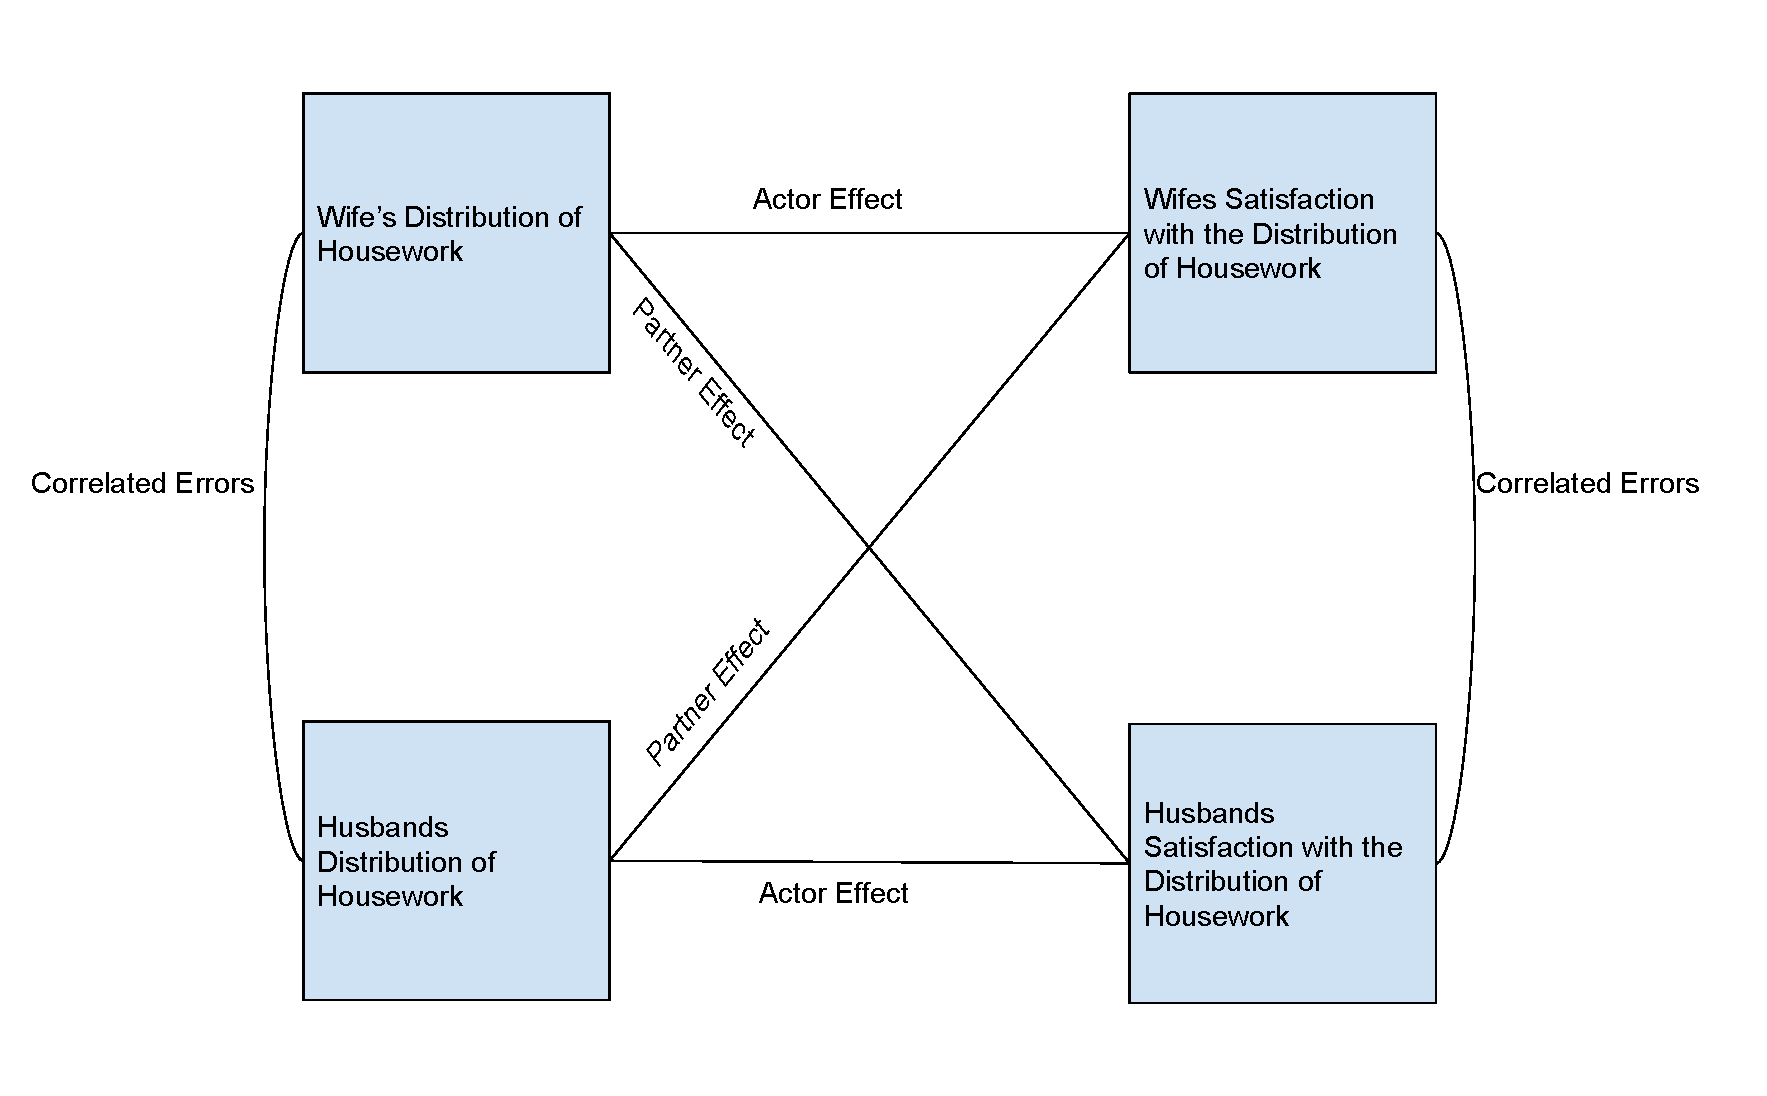
\includegraphics{APIM_Housework_Distribution.pdf}
<<<<<<< HEAD
\#\# Main Results

Looking at the summary table above, the only relationship that is statistically significant is the one between the wife's satisfaction level and her average housework. We know this because the p-value for \texttt{as.factor(genderE\_A)1:Cavg\_housework\_female\_A} is 0.0041, which is less than 0.05. Since the value for this relationship is -0.029132, it signifies that as the wife's average housework increases, her satisfaction level decreases.

For women, her gender role beliefs significantly moderated the relationship between her own housework distribution and her satisfaction with the housework distribution. The moderation effect was 0.07 with a p value of \textless0.05 and a standard deviation of 0.02. For every one unit increase in gender role beliefs, satisfaction increases by 0.07 while keeping housework distribution constant.Again for women, her partners gender role beliefs significantly moderated the relationship between her own housework distribution and her satisfaction with the housework distribution. The moderation effect was -0.06 with a p value of 0.01 and a standard deviation of 0.02. For every one unit increase in her partners gender role beliefs, her own satisfaction increases by -0.06 while keeping housework distribution constant.

Looking at the summary table above, these are the relationships that are statistically significant: as.factor(genderE\_A)1:Cavg\_housework\_female\_A:Cavg\_grbs\_P, 8.742833e-03
=======
\caption{\label{fig:my-figure}Actor Partner Effects in the APIM}
\end{figure}

\hypertarget{main-results}{%
\subsection{Main Results}\label{main-results}}

\hypertarget{gender-role-beliefs}{%
\subsubsection{Gender Role Beliefs}\label{gender-role-beliefs}}

Looking at the summary table above, the only relationship that is statistically significant is the one between the wife's satisfaction level and her average housework. We know this because the p-value for \texttt{as.factor(genderE\_A)1:Cavg\_housework\_female\_A} is 0.0041, which is less than 0.05. Since the value for this relationship is -0.029132, it signifies that as the wife's average housework increases, her satisfaction level decreases.

For women, her gender role beliefs significantly moderated the relationship between her own housework distribution and her satisfaction with the housework distribution. The moderation effect was 0.07 with a p value of \textless0.05 and a standard deviation of 0.02. For every one unit increase in her gender role beliefs, her satisfaction increases by 0.07 while keeping housework distribution constant. Again for women, her partners gender role beliefs significantly moderated the relationship between her own housework distribution and her satisfaction with the housework distribution. The moderation effect was -0.06 with a p-value of 0.01 and a standard deviation of 0.02. For every one unit increase in her partners gender role beliefs, her own satisfaction increased by -0.06 while keeping housework distribution constant.

Looking at the summary table above, these are the relationships that are statistically significant:
as.factor(genderE\_A)1:Cavg\_housework\_female\_A:Cavg\_grbs\_P, 8.742833e-03
>>>>>>> 71ff8d82663603c79f5ff4fcd38ff2052482afae
as.factor(genderE\_A)1:Cavg\_housework\_female\_A:Cavg\_grbs\_A, 8.408625e-04
as.factor(genderE\_A)0:Cavg\_housework\_female\_A, 2.259373e-02

Only looking at the three way interactions with gender we found two significant gender differences in the moderation effects. The interaction between actors housework distribution and their own gender role beliefs was significantly different for husbands and wives with an estimate of 0.06 a p value of 0.03 and a standard deviation of 0.03. The moderation effect of ones own gender role beliefs was 0.06 units higher for women than men meaning the moderation effect of gender role beliefs had a significantly larger positive effect on satisfaction for wives than for husbands.
<<<<<<< HEAD
In addition the interaction between actors housework distribution and their partners gender role beliefs was significantly different for husbands and wives with an estimate of -0.08 a p value of 0.01 and a standard deviation of 0.03.The moderation effect of ones partners gender role beliefs was -0.08 units lower for women than men meaning the moderation effect of her husbands gender role beliefs had a significantly larger negative effect on satisfaction compared to how her gender role beliefs effected the relationship between housework distribution and satisfaction for her husband.






=======

In addition the interaction between actors housework distribution and their partners gender role beliefs was significantly different for husbands and wives with an estimate of -0.08 a p-value of 0.01 and a standard deviation of 0.03.The moderation effect of ones partners gender role beliefs was -0.08 units lower for women than men meaning the moderation effect of her husbands gender role beliefs had a significantly larger negative effect on satisfaction compared to how her gender role beliefs effected the relationship between housework distribution and satisfaction for her husband.

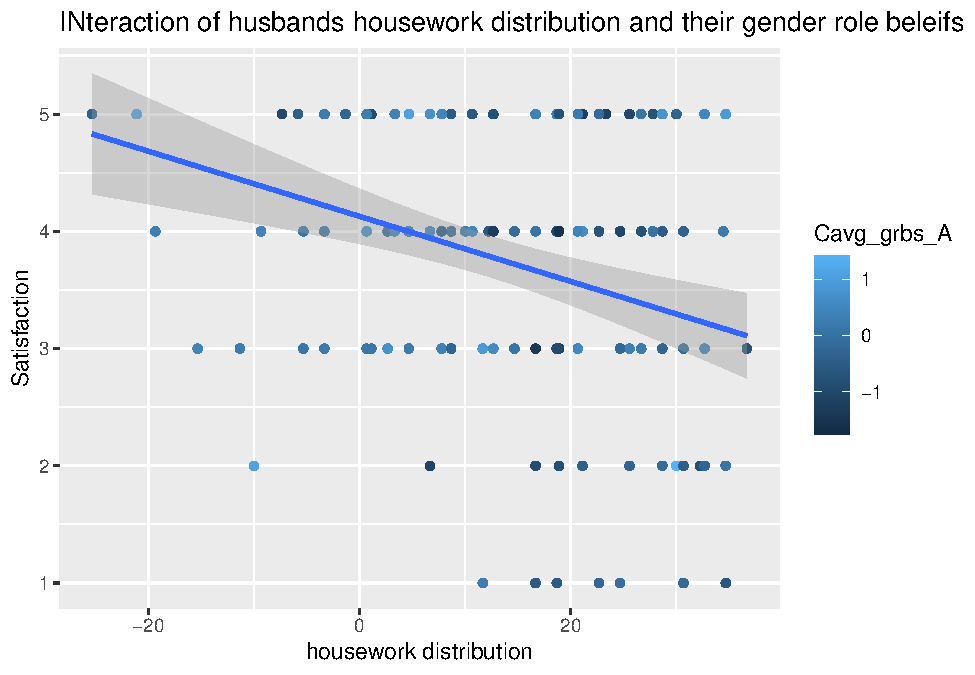
\includegraphics{results_files/figure-latex/unnamed-chunk-9-1.pdf}
As the housework distribution increases for wives with low gender role beliefs, their satisfaction decreases. This makes sense because wives with low gender role beliefs would believe in an equal housework distribution where she wasn't doing majority of the housework tasks. As the housework distribution increases for wives with high gender role beliefs, their satisfaction has a very slight decrease, but it stays more or less the same.

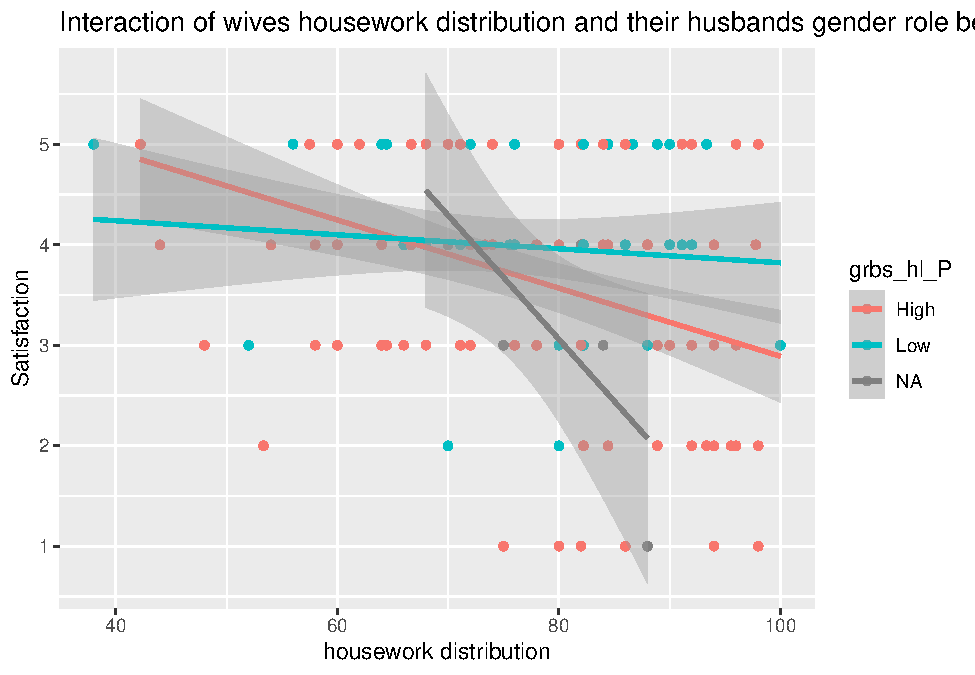
\includegraphics{results_files/figure-latex/unnamed-chunk-10-1.pdf}

As the housework distribution increases for wives whose husbands have low gender role beliefs, their satisfaction remains constant. As the housework distribution increases for wives whose husbands have high gender role beliefs, their satisfaction decreases.

\hypertarget{religion}{%
\subsubsection{Religion}\label{religion}}
>>>>>>> 71ff8d82663603c79f5ff4fcd38ff2052482afae

The two intercept model gives us the two coefficients for men and women

\hypertarget{exploratory-results}{%
\subsection{Exploratory Results}\label{exploratory-results}}

\begin{itemize}
\tightlist
\item
  one more diagram
\end{itemize}

We want to explore the possibility of gatekeeping being a significant factor in our analysis. Are women with higher gender role beliefs more likely to gatekeep housework tasks?


\clearpage
\renewcommand{\listfigurename}{Figure captions}

\clearpage
\renewcommand{\listtablename}{Table captions}


\end{document}
